% !TeX spellcheck=en_GB
\section{Results}

This section contains our benchmarking results as well as a discussion of the results.

For each of the test categories, we measure performance for the three parallel versions, the outer parallel version executed sequentially on the CPU, and the sequential CPLEX java program. We have chosen instance sizes based on what could finish within at most a few minutes on our systems. The programs mentioned in Section \ref{priorwork} were typically tested on larger instances, but with a run-time of tens of minutes or even hours.

We plot the times in the same graphs for comparison. Note that comparison between the sequential and parallel versions might not be meaningful since they are executed on different machines and architectures. Additionally, different graphs should not be compared to each other as they use different scales.
\clearpage

\subsection{One big instance}
In this test category, we vary the size of the linear program while keeping the number of instances constant at one.

\begin{figure}[H]
	\centering
	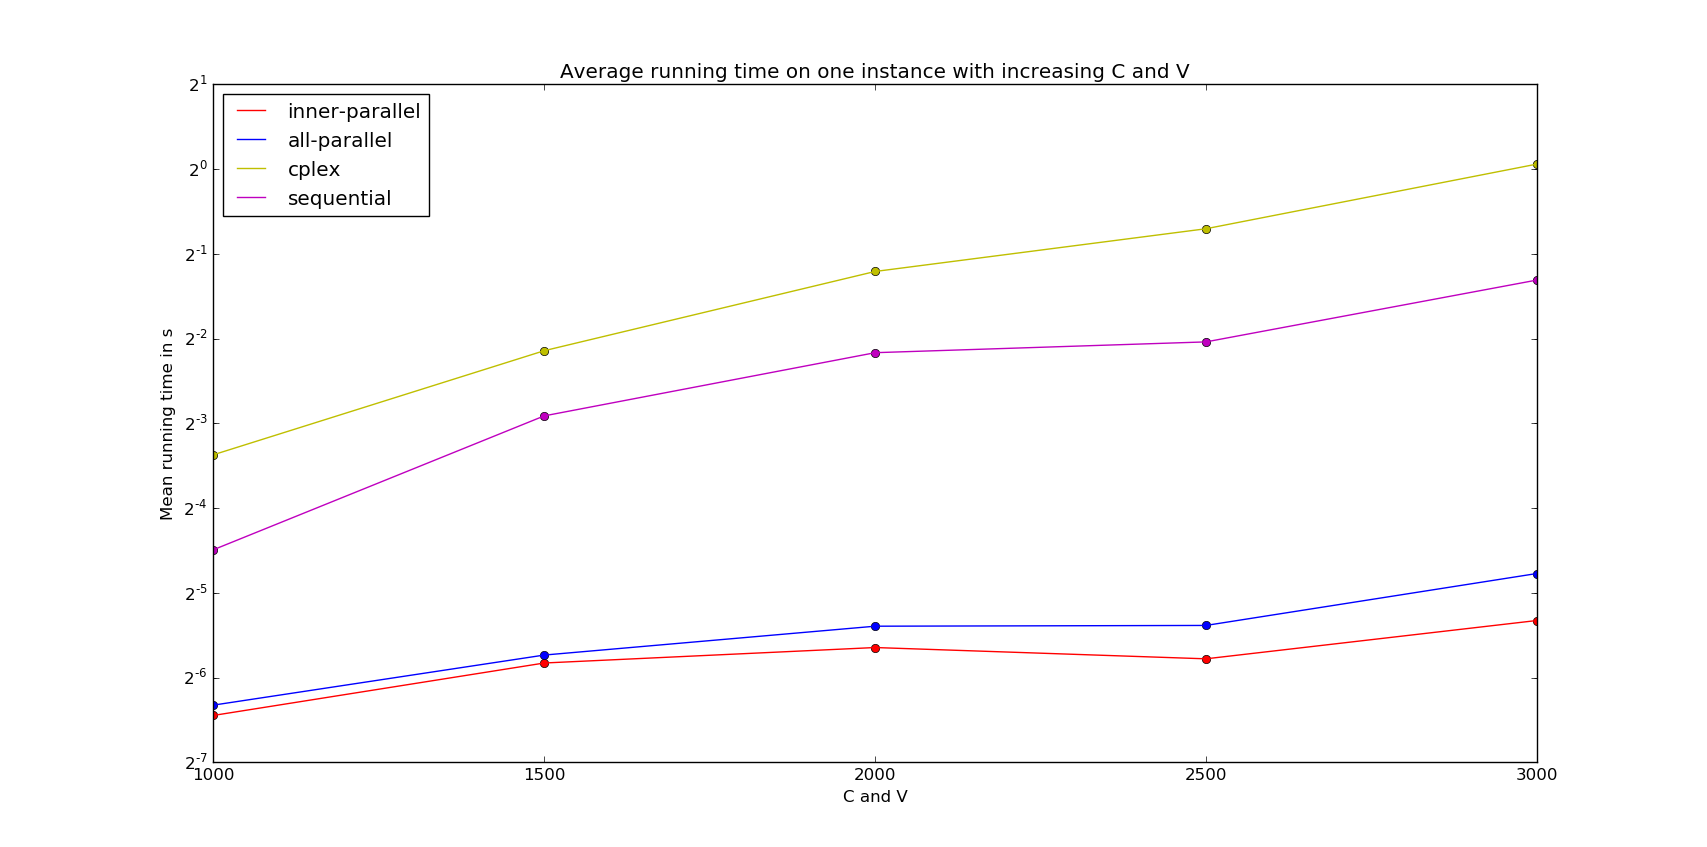
\includegraphics[width=\textwidth]{one-big}
	\caption{The average running time in seconds of the different implementations, with one instance with $m$ and $n$ going from 1000 to 5000. Note that the sequential and outer-parallel are not part of this graph as they were not computed due to running time.}
	\graphicspath{dir-list}
	\label{fig:one}
\end{figure}

As seen in Figure \ref{fig:one}, the CPLEX version is the fastest implementation across all tested versions. This is expected since it is the current state of the art method. Its running time appears to scale linearly with the size of the instance.

The inner and fully parallel versions are somewhat comparable with each other, although they might diverge further for larger instances. We would expect the inner parallel version to be the fastest of the two as it has less overhead. Both versions arre fully parallel on one instance, which would indicate the iterations in the convergence loop dominate the performance. Both seem to be scaling exponentially.

The outer parallel version both on the GPU and the CPU (our sequential baseline) are not shown on the graph, because their performance were significantly worse than the others and took too long to finish.
\clearpage

\subsection{Many small instances}

In this test category, we vary the number of instances while keeping the sizes within a constant range of low values.

\begin{figure}[H]
	\centering
	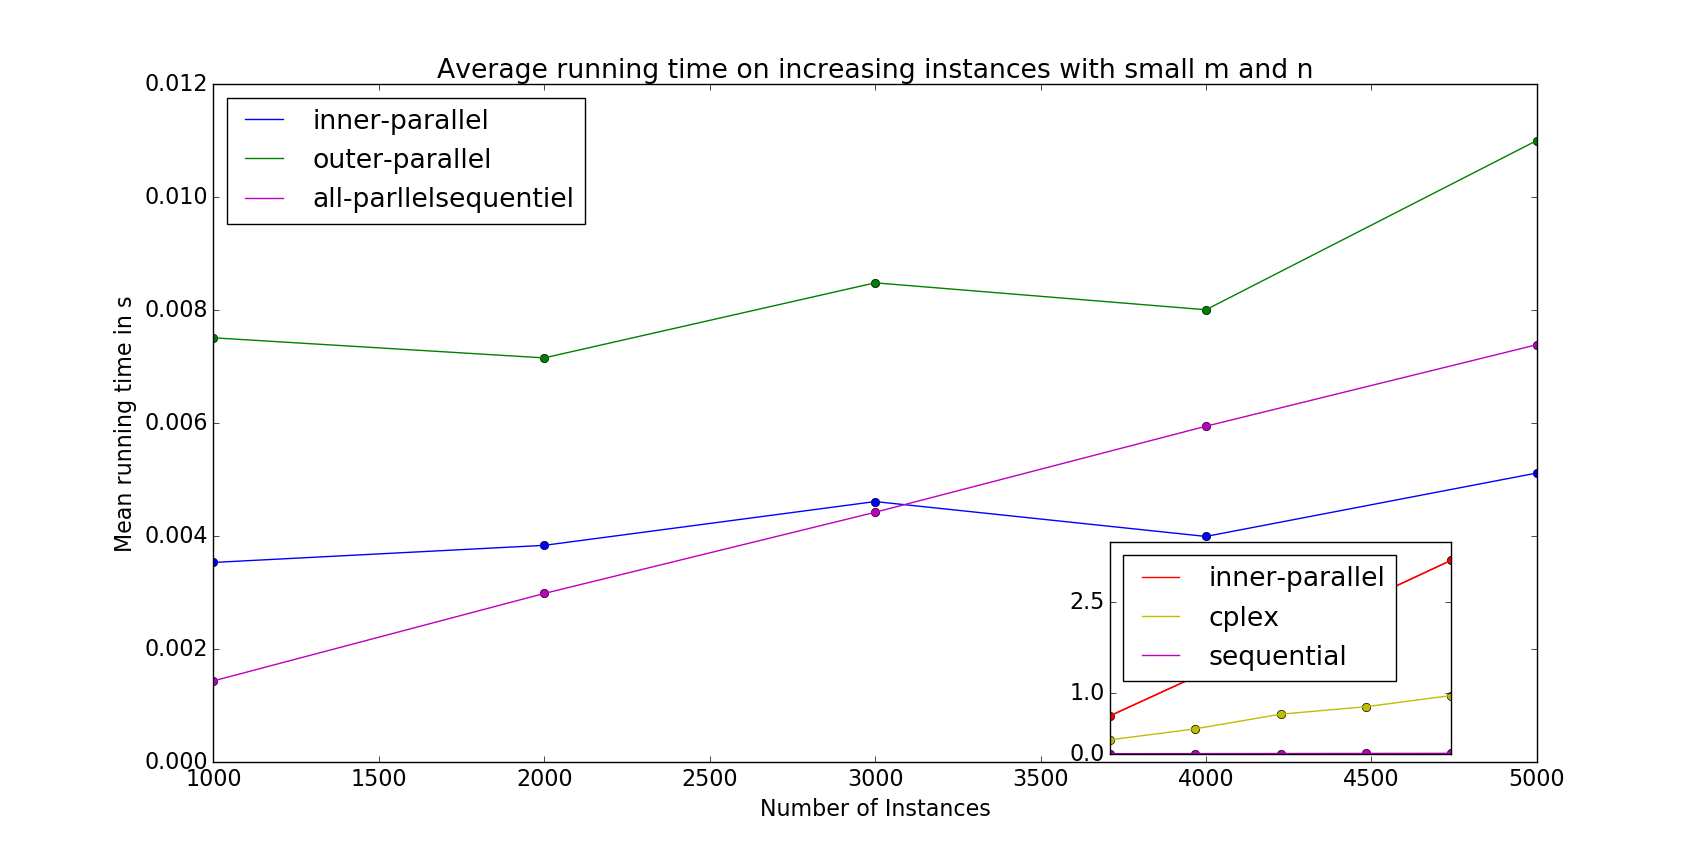
\includegraphics[width=\textwidth]{many-small-in-one}
	\caption{The average running time of the different implementations, on different number of instances with $m$ and $n$ in a range between 1 and 10. The little graph shows the difference between
  the inner parallel version and cplex version. The purple line is where the three others have their running time.}
	\graphicspath{dir-list}
	\label{fig:small}
\end{figure}

As seen on Figure \ref{fig:small} the outer parallel version is the fastest for the largest number of instances. This is expected since it is parallel on the outer dimension, which is the dominant dimension in these test cases. The sequential version is the fastest for fewer than 3000 instances, but it has a more steep upwards slope, indicating that its growth might also exceed the fully parallel version.

Since each instance only requires relatively little work, the inner parallel version performs poorly. The fully parallel version performs well, which is expected since it is also parallel in the outer dimension, but it is clear that the overhead for flattening the nested parallelism makes it slower than the only outer parallel version.

CPLEX performs badly here which is possibly due to the pure overhead in solving a single instance. We also note that the assumptions in our implementations are not present in CPLEX. This could result in extra constant-time overhead for CPLEX per instance.
\clearpage

\subsection{Many big instances}
In this test category, we vary the number of instances while keeping the sizes within a constant range of high values.

\begin{figure}[H]
	\centering
	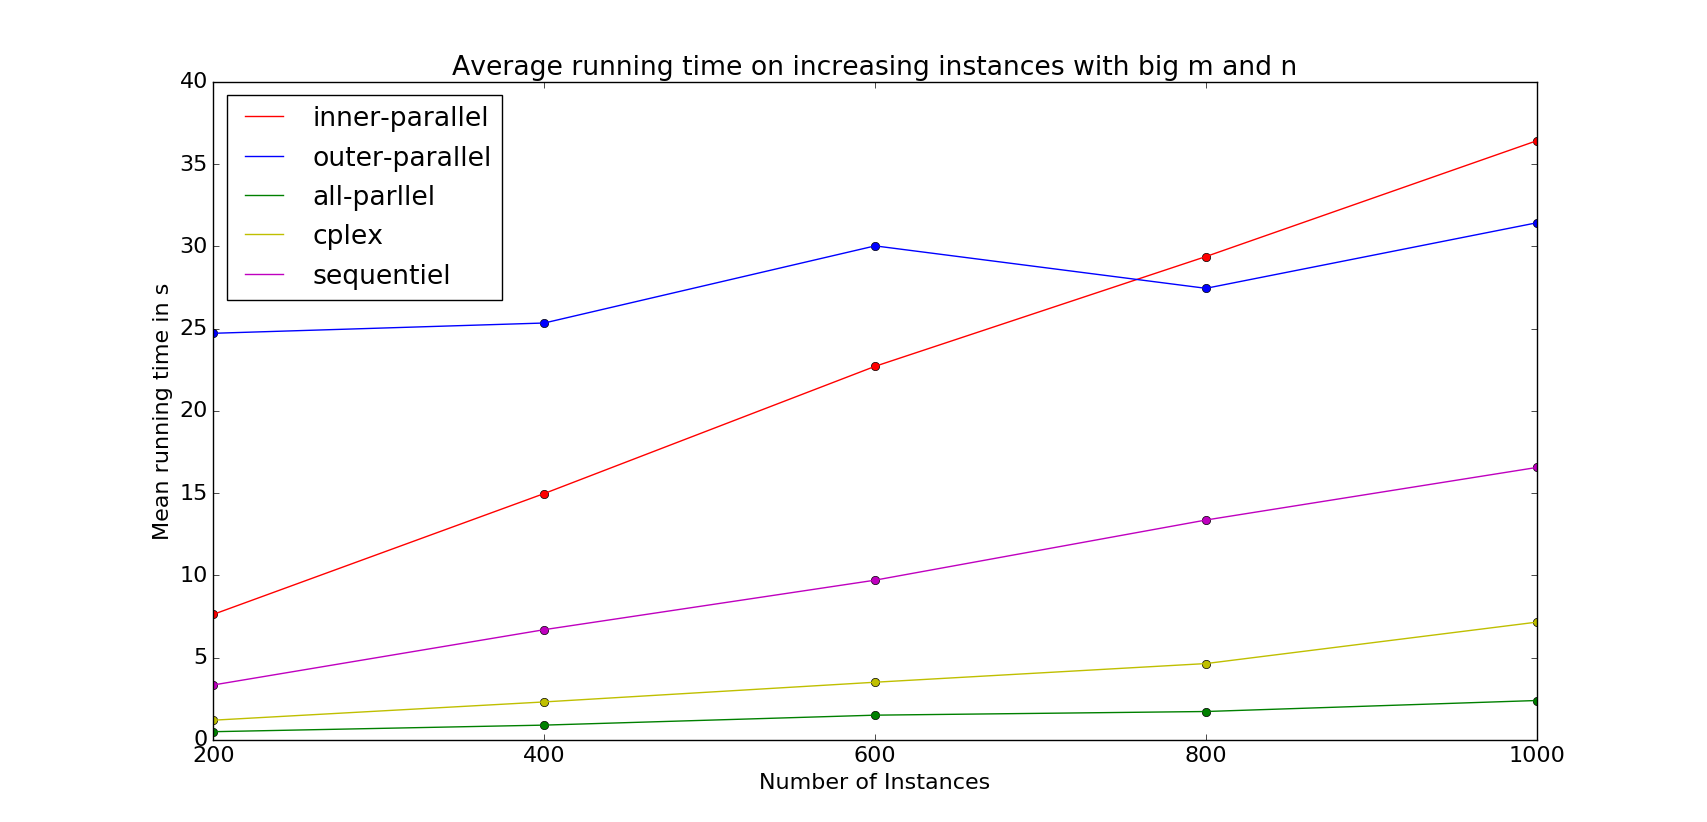
\includegraphics[width=\textwidth]{many-big}
	\caption{The average running time of the different implementations, on different sizes of instances, with high numbers of $m$ and $n$ in a range between 150 and 200.}
	\graphicspath{dir-list}
	\label{fig:big}
\end{figure}

As seen in Figure \ref{fig:big} the fully parallel implementation is the fastest. This was expected since it is the implementation with the highest level of parallelism on both dimensions. Since both dimensions are large, it effectively utilises the number of threads to its fullest and the overhead becomes negligible.

The CPLEX version is not far behind. If the instances were solved concurrently, it is possible that it would be faster than the fully parallel GPU version. The inner and outer parallel versions do not perform well, likely because they are blocked on the dimension on which they are not parallel.
\clearpage

\subsection{Many instances of varying size}
In this test category, we vary the number of instances while keeping the sizes within a constant, but broad range of values.

\begin{figure}[H]
	\centering
	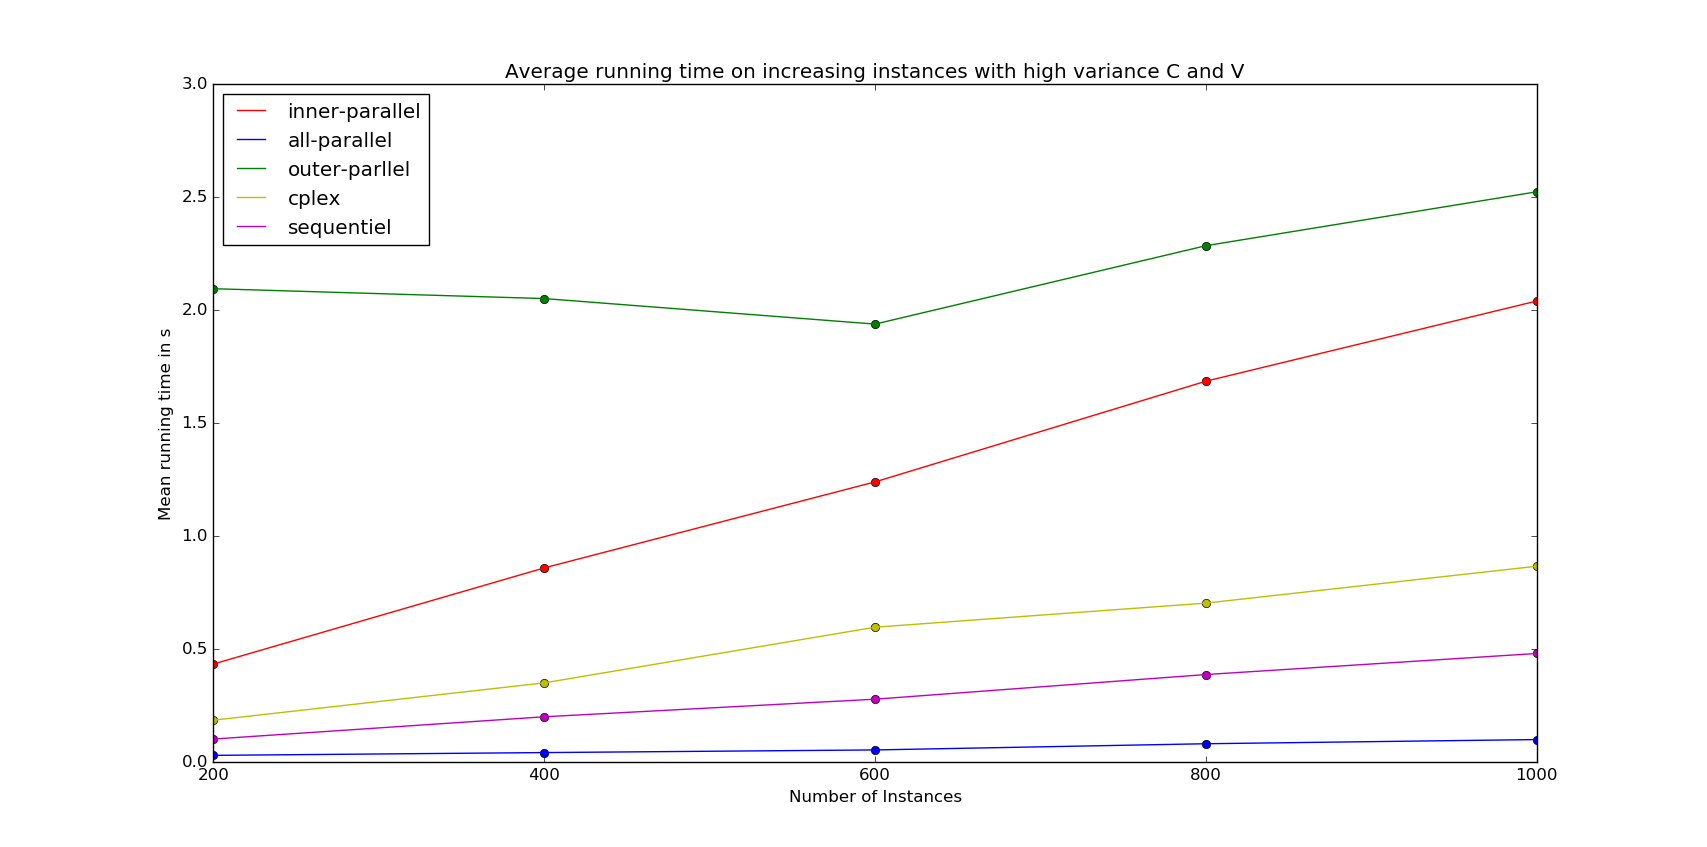
\includegraphics[width=\textwidth]{many-varying}
	\caption{The average running time of the different implementations, on different sizes of instances, with $m$ and $n$ in a range between 10 and 150.}
	\graphicspath{dir-list}
	\label{fig:vary}
\end{figure}

As seen in Figure \ref{fig:vary} the fully parallel version shows its strength. As in the category with many big instances, it is capable of maintaining high GPU utilisation without getting bottlenecked.

Again, as in the many big instances category, the inner and outer parallel versions perform the worst. However, the outer and fully parallel versions have almost constant running time as the number of instances increase. This could indicate that they are both blocked on the deepest instance while solving all other instances simultaneously. The outer parallel version is just slower because it is not parallel on a single instance.

Meanwhile, the inner parallel version scales linearly with a much higher constant than the sequential versions. We would expect it to scale linearly, as it computes all instances in sequence. The high constant could be due to the overhead of executing on the GPU without being able to take much advantage of it.